% TEMPLATE for Usenix papers, specifically to meet requirements of
%  USENIX '05
% originally a template for producing IEEE-format articles using LaTeX.
%   written by Matthew Ward, CS Department, Worcester Polytechnic Institute.
% adapted by David Beazley for his excellent SWIG paper in Proceedings,
%   Tcl 96
% turned into a smartass generic template by De Clarke, with thanks to
%   both the above pioneers
% use at your own risk.  Complaints to /dev/null.
% make it two column with no page numbering, default is 10 point

% Munged by Fred Douglis <douglis@research.att.com> 10/97 to separate
% the .sty file from the LaTeX source template, so that people can
% more easily include the .sty file into an existing document.  Also
% changed to more closely follow the style guidelines as represented
% by the Word sample file. 
% This version uses the latex2e styles, not the very ancient 2.09 stuff.
\documentclass[letterpaper,twocolumn,10pt]{article}
\usepackage{usenix,epsfig,endnotes,xspace}

% Name candidates:
%  Anza
%  Void 
%  Station (from Genesis's "Grand Central" component) 
%  TARDIS: Atomic, Recoverable, Datamodel Independent Storage

\newcommand{\yad}{Void\xspace}
\newcommand{\oasys}{Juicer\xspace}

\newcommand{\eab}[1]{\textcolor{red}{\bf EAB: #1}}
\newcommand{\rcs}[1]{\textcolor{green}{\bf RCS: #1}}
\newcommand{\mjd}[1]{\textcolor{blue}{\bf MJD: #1}}

\begin{document}

%don't want date printed
\date{}


%make title bold and 14 pt font (Latex default is non-bold, 16 pt)
\title{\Large \bf \yad: A Terrific Application and Fascinating Paper}

%for single author (just remove % characters)
\author{
{\rm Russell Sears}\\
UC Berkeley
\and
{\rm Michael Demmer}\\
UC Berkeley
\and
{\rm Eric Brewer}\\
UC Berkeley
} % end author

\maketitle

% Use the following at camera-ready time to suppress page numbers.
% Comment it out when you first submit the paper for review.
%\thispagestyle{empty}


\subsection*{Abstract}

\yad is a storage framework that incorporates ideas from traditional
write-ahead-logging storage algorithms and file system technologies,
while providing applications with increased control over its
underlying modules.  Generic transactional storage systems such as SQL
and BerkeleyDB serve many applications well, but impose constraints
that are undesirable to developers of system software and
high-performance applications.  Conversely, while filesystems place
few constraints on applications, the do not provide atomicity or
durability properties that naturally correspond to application needs.

This paper addresses this gap (and enables the development of
unforeseen variants on transactional storage) by generalizing
write-ahead-logging algorithms.  Our partial implementation of these
ideas already provides specialized (and cleaner) semantics and
improved performance to applications.

%Applications may use our modular library of basic data strctures to
%compose new concurrent transactional access methods, or write their
%own from scratch.  
This paper presents examples that make use of custom access methods,
modifed buffer manager semantics, direct log file manipulation, and
LSN-free pages that facilitate zero-copy optimizations, and discusses
the composability of these extensions.

We argue that our ability to support such a diverse range of
transactional systems stems directly from our rejectiion of
assumptions made by early database designers.  These assumptions
permeate ``database toolkit'' research.  We attribute the success of
low-level transaction processing libraries (such as Berkeley DB) to
a partial break from traditional database dogma.

% entries, and 
% to reduce memory and
%CPU overhead, reorder log entries for increased efficiency, and do
%away with per-page LSNs in order to perform zero-copy transactional
%I/O.  
%We argue that encapsulation allows applications to compose
%extensions.

%These ideas have been partially implemented, and initial performance
%figures, and experience using the library compare favorably with
%existing systems.


\section{Introduction}

%It is well known that, to a system implementor, high-level
%abstractions built into low-level services are at best a nuisance, and
%often lead to the circumvention or complete reimplementation of
%complex, hardware-dependent code.

%This work is based on the premise that as reliability and performance
%issues have forced ``low-level'' operating system software to
%incorporate database services such as durability and isolation.  As
%this has happened, the abstractions provided by database systems have
%seriously restricted system designs and implementations.

Approximately a decade ago, the operating systems research community came to
the painful realization that the presence of high level abstractions
in ``unavoidable'' system components precluded the development of
crucial, performance sensitive applications.~\cite{exterminate, stonebrakerDatabaseDig}

As our reliance on computing infrastructure has increased, components
for the reliable storage and manipulation of data have become
unavoidable.  However, current transactional storage systems provide
abstractions that are intended for systems that execute many
independent, short, and computationally inexpensive progams
simultaneously.  Modern systems that deviate from this description are
often forced to use existing systems in degenerate ways, or to
reimplement complex, bug-prone data manipulation routines by hand.

%Examples include:
%\begin{itemize}
%\item Search engines
%\item Document repositories (including desktop search)
%\item Web based email services
%\item Web based map and gis services
%\item Ticket reservation systems
%\item Photo, audio and video repositories
%\item Bioinformatics
%\item Version control systems
%\item Workflow applications
%\item CAD/VLSI applications
%\item Directory services
%\end{itemize}

Examples of real world systems that currently fall into this category
are web search engines, document repositories, large-scale web-email
services, map and trip planning services, ticket reservation systems,
photo and video repositories, bioinformatics, version control systems,
workflow applications, CAD/VLSI applications and directory services.

Applications that have only recently begun to make use of high-level
database features include XML based systems, object persistance
mechanisms, and enterprise management systems (notably, SAP R/3).

In short, we believe that a fundamental architectural shift in
transactional storage is necessary before general purpose storage
systems are of practical use to modern applications.
Until this change occurs, databases' imposition of unwanted
abstraction upon their users will restrict system designs and
implementations.

%To paraphrase a hard-learned lesson the operating sytems community:
%
%\begin{quote} The defining tragedy of the [database] systems community
%  has been the definition of an [databse] system as software that both
%  multiplexes and {\em abstracts} physical resources...The solution we
%  propose is simple: complete elimination of [database] sytems
%  abstractions by lowering the [database] system interface to the
%  hardware level~\cite{engler95}.
%\end{quote}

%In short, reliable data managment has become as unavoidable as any
%other operating system service.  As this has happened, database
%designs have not incorporated this decade-old lesson from operating
%systems research:
%
%\begin{quote} The defining tragedy of the operating systems community
%  has been the definition of an operating system as software that both
%  multiplexes and {\em abstracts} physical resources...The solution we
%  propose is simple: complete elimination of operating sytems
%  abstractions by lowering the operating system interface to the
%  hardware level~\cite{engler95}.
%\end{quote}


The widespread success of lower level transactional storage libraries
(such as Berkeley DB) is a sign of these trends.  However, the level
of abstraction provided by these systems is well above the hardware
level, and applications that resort to ad-hoc storage mechanisms are
still common.

This paper presents \yad, a library that provides transactional
storage at a level of abstraction as close to the hardware as
possible.  The library can support special purpose, transactional
storage interfaces as well as ACID, database style interfaces to
abstract data models.  

Notably, \yad incorporates many existing technologies from the storage
communities, and allows applications to incorporate appropriate
subsystems as necessary.  A partial open-source implementation of the
ideas presented below is available; performance numbers are provided
when possible.

**We've explained why the sky is falling.  Now, explain why \yad is
so good.  (Take ideas from old paper.)**

\section{Prior work}

Database research has a long history, including the development of
many technologies that our system builds upon.  However, we view \yad
as a rejection of the fundamental assumptions that underly database
systems.  In particular, we reject the idea that a general purpose
storage sytem should attempt to encode universal data models and
computational paradigms.  

Instead, we are less ambitious and seek to build a storage system that
provides durable (which often implies transactional) access to the
primitives provided by the underlying hardware.  To be of practical
value, it must be easy to specialize such a system so that it encodes
any of a variety of data models and computational paradigms.
Otherwise, the system could not easily reused in many environments.
We know of no system that adequately achieves these two goals.

Here, we present a brief history of transactional storage systems, and
explain why they fail to achieve \yad's goals.  Citations of the
technical work upon which our system is based are included below, in
the description of \yad's design.

%Here we will focus on lines of research that are
%superficially similar, but distinct from our own, and cite evidence
%from within the database community that highlights problems with
%systems that attempt to incorporate databases into other systems.

%Of course, database systems have a place in modern software
%development and design, and are the best available storage solution
%for many classes of applications.  Also, this section refers to work
%that introduces technologies that are crucial to \yad's design; when
%we claim that prior work is dissimilar to our own, we refer to
%high-level architectural considerations, not low-level details.

\subsection{Databases  as system components}

A recent survey~\cite{riscDB} enumerates problems that plague users of
state-of-the-art database systems.  It concludes that efficiently optimizing and
consistenly servicing large declarative queries is inherently
difficult.  

The survey finds that database implementations fail to support the needs of modern systems.  
In large systems, this manifests itself as managability and tuning issues that
prevent databases from effectively servicing large scale, diverse, interactive
workloads.  
On smaller systems, footprint, predictable performance, and power
consumption are primary concerns, that are not addressed by full-fledged database systems.
Database applications that must scale up to large numbers of independent, self-administering desktop 
installations will be problematic unless a number of open research problems are solved.  

The survey also provides evidence that SQL itself is problematic.  
While SQL serves some classes of applications well, it is
often inadequate for algorithmic and hierarchical computing tasks.

Finally, complete, modern database
implementations are often incomprehensible, and border on
irreproducable, hindering further research.  After making these
points, the study concludes by suggesting the adoption of ``RISC''
style database architectures, both as a research and as an
implementation tool~\cite{riscDB}.  

%For example, large scale application such as web search, map services,
%e-mail use databases to store unstructured binary data, if at all.

%More recently, WinFS, Microsoft's database based
%file metadata management system, has been replaced in favor of an
%embedded indexing engine that imposes less structure (and provides
%fewer consistency guarantees) than the original
%proposal~\cite{needtocitesomething}.

%Scaling to the very large doesn't work (SAP used DB2 as a hash table
%for years), search engines, cad/vlsi didn't happen.  scalable GIS
%systems use shredded blobs (terraserver, google maps), scaling to many
%was more difficult than implementing from scratch (winfs), scaling
%down doesn't work (variance in performance, footprint),

\subsection{Database Toolkits}

\yad is a library that could be used to provide the storage primatives needed by a
database server.  Therefore, one might suppose that \yad is a database
toolkit.  However, such an assumption would be incorrect, as \yad incorporates neither of the two basic concepts that underly database toolkit designs.  These two concepts are 
{\em conceptual-to-internal mappings}~\cite{batoryConceptual}
and {\em physical database models}~\cite{batoryPhysical}.

Conceptual-to-internal mappings and physical database models were
discovered during an early survey of database implementations.  Mappings
desribe the computational primitives upon which client applications must 
be implemented.  Physical database models define the on-disk layout used 
by a system in terms of data layouts and representations that are commonly 
used by relational and navigational database implementations.

Both concepts are fundamentally incompatible with a general storage
implementation.  By definition, a database server encodes both
concepts, while transaction processing libraries mange to avoid
conceptual mappings. \yad's novelty stems from the fact that it avoids
both concepts, while making it easy for applications to incorporate results from the database
literature.


\subsubsection{Conceptual mappings}

%Database toolkits are based upon the idea that database
%implementations can be broken into smaller components with
%standardized interfaces.  

%Early work in this field surveyed database
%implementations that existed at the time.  It casts compoenents of
%these implementation in terms of a physical database
%model~\cite{batoryPhysical} and conceptual-to-internal
%mappings~\cite{batoryConceptual}.  These abstractions describe
%relational database systems, and describe many aspects of subsequent
%database toolkit research.

%However, these abstractions are built upon assumptions about
%application structure and data layout.  

At the time of their introduction, ten
conceptual-to-internal mappings were sufficient to describe existing
database systems.  These mappings included indexing, encoding
(compression, encryption, etc), segmentation (along field boundaries),
fragmentation (without regard to fields), $n:m$ pointers, and
horizontal partitioning, among others.
  
The initial survey postulates that a finite number of such mappings
are adequate to describe database systems.  A 
database toolkit need only implement each type of mapping in order to
encode the set of all conceivable database systems.

Our work's primary concern is to support systems beyond database
implementations.  If we were to follow the database toolkit approach,
we would proceed by developing a framework that adequately encodes the
set of all abstract data types and all algorithms that system software
designers make use of.  Finally, we would describe a framework that is
capable of encoding all conceivable system software designs, and
encode stanadard, intechangable interfaces to each type of component
in our framework.

Put this way, the database toolkit approach to system design seems
absurd.  However, similar approachs have been extremeley successful
for well-understood, well-defined classes of applications.  In
particular, it has been highly successful in the design of systems
that perform limited types of computations over particular classes of
data.  Much of the database literature is based upon this idea, and
continues to successfully improve the state of computer science, and
is the basis of the highly sucessful database industry.  

Clearly, however, this approach is inappropriate for the design of
general purpose components for system developers, or for applications
that make use of unique computational and storage primitives.
Therefore, \yad's architecture avoids hard-coded assumptions regarding
the computation or abstract data types of the applications built on
top of it.

Instead, it leaves decisions regarding abstract data types and
algorithm design to system developers or language designers.  For
instance, while \yad has no concept of object oriented data types, two
radically different approaches toward object persistance have been
implemented on top of it.~\ref{oasys}

We could have just as easily written a persistance mechanism for a
functional programming language, or a particular application (such as
an email server).  Our experience building data manipulation routines
on top of application-specific primitives was favorable compared to
past experiences attempting to restructure entire applications to
match pre-existing computational models, such as SQL's declarative
interface.

\subsubsection{Physical data models}

As it was initially tempting to say that \yad was a database toolkit,
it may now be tempting to claim that \yad implements a physical
database model.  In this section, we discuss fundamental limitations
of the physical data model, and explain how \yad avoids these
limitations.  

We discuss Berkeley DB, and show that it provides funcationality
similar to a physical database model.  Just as \yad allows
applications to build mappings on top of the primitives it provides,
\yad's design allows them to take design storage in terms of a
physical database model.  Therefore, while Berkeley DB could be implemented on top
of \yad, Berkeley DB cannot support the primitives provided by \yad.

Genesis,~\cite{genesis} an early database toolkit, was built in terms
of interchangable primitives that implemented the interfaces of an
early database implementation model.  It built upon the idea of
conceptual mappings described above, and the physical database model
decribed here.

The physical database model provides the abstraction upon which
conceptual mappings can be built.  It is based on a partitioning of storage into 
{\em simple files}, which provide operations associated with key based storage, and
{\em linksets}, which make use of various pointer storage schemes to provide
mappings between records in simple files~\cite{batoryPhysical}.  

Subsequent database toolkit work builds upon these foundations,
Exodus~\cite{exodus} and Starburst~\cite{starburst} are notable
examples, and incorporated a number of ideas that will be referred to
later in this paper.  Although further discussion is beyond the scope
of this paper, object oriented database systems, and relational
databases with support for user definable abstract data types (such as
in Postgres~\cite{postgres}) were the primary competitors to these
database toolkits work.

Fundamentally, all of these systems allowed users to quickly define
new DBMS software by defining some abstract data types and often index
methods to manipulate these types.  Data was adressable via various
mechanisms.  Most systems implemented a particular addressing scheme
(direct, hash based, tree based, etc), depending on the applications
it supported.  Many potential linkset implementations exist, each
targets a particular workload.  More complex data strucutres (such as
graphs) could be built on these primitives.  Some systems optimized
for fast pointer traversal, making it impractical to rearrange data on
disk after allocation, while others interposed an expensive index
lookup on each pointer traversal.  Special purpose optimizations were
added, addressing egregious performance issues that were exposed by
common workloads built on common sets of tradeoffs.  This process
leads to highly complex physical database designs that implement a
compromise between applications with widely varying needs.

Furthermore the features and abstractions that introduce this complexity 
are designed to efficiently serve the needs of a database implementation.  
As \yad seeks to address applications not well serviced by database
systems, the value of these features is dubious, especially if they
are provided as a monolithic physical database implementation.

Therefore, \yad abandons the concept of a physical database.  Instead
of forcing applications to reason in terms of simple files and
linksets, it allows applications to reason about storage in terms of
atomically applicable changes to the page file.  Of course,
applications that wish to reason in terms of linksets and simple files
are free to do so.

We reget forcing applications to arrange for updates to be atomic, but
this restriction is fundamental if we wish to support concurrent
transactions, durability and recovery using conventional hardware
systems.  In Section~\ref{nestedTopActions} we explain how a set of
atomic changes may be atomically applied to the page file, alleviating
the burden we place upon applications somewhat.

Now that we have introduced the underlying concepts of database 
toolkits, we can discuss the proposed RISC database architectures 
in more detail.  RISC databases have many elements in common with
database toolkits.  However, they take the database toolkit idea one
step further, and suggest standardizing the interfaces of the
toolkit's internal components, allowing multiple organizations to
compete to improve each module.  The idea is to produce a research
platform, and to address issues that affect modern
databases, such as automatic performance tuning, and reducing the
effort required to implement a new database system~\cite{riscDB}.

While we agree with the motivations behind RISC databases, instead of
building a modular database, we seek to build a module that allows
programmers to avoid databases.


\subsection{Transaction processing libraries}

Berkeley DB is a highly successful alternative to conventional
database design.  At its core, it provides the physical database, or
relational storage system of a conventional database server.

This module focuses on providing fully transactional data storage with
B-Tree and hashtable based indexes.  Berkeley DB also provides some
support for application specific access methods, as did Genesis, and
the database toolkits that succeeded it.~\cite{libtp} Finally,
Berkeley DB allows applications that need to modify the recovery
semantics of Berkeley DB, or otherwise tweak the way its
write-ahead-logging protocol works to pass flags via its API.

Transaction processong libraries are \yad's closest relative.
However, \yad provides applications with a broader range of options
for tweaking, customizing, or completely replacing each of the
primitives it uses to implement write-ahead-logging.  

The current \yad implementation includes sample implementations of Berkeley
DB style functionality, but the use of this functionality is optional.
Later in the paper, we provide examples of how this functionality and
the write-ahead-logging algorithm can be modified to provide
customized semantics to applications, while improving overall system
performance.  

The Boxwood system provides a networked, fault-tolerant transactional
B-Tree and ``Chunk Manager.''  We believe that \yad could be a
valuable part of such a system, especially given \yad's focus on
intelligence and optimizations within a single node.  In particular,
when implementing applications with predictable locality properties, 
it would be interesting to explore alternative approaches toward the
implementation of Boxwood that make use of \yad's customizable
write-ahead-logging semantics, and fully logical logging mechanism.


%  This part of the rant belongs in some other paper:
%
%Offer rebuttal to the Asilomar Report.  On the web 2.0, no one knows
%you implemeneted your web service with perl and duct tape...  Is it
%possible to scale to 1,000,000's of datastores without punting on the
%data model?  (HTML suggests not...) Argue that C bindings are be the
%�universal glue� the RISC db paper should be asking for.

%cover P2 (the old one, not "Pier 2" if there is time...

\section{Write ahead loging}

This section describes how \yad uses write-ahead-logging to support the
four properties of transactional storage: Atomicity, Consistency,
Isolation and Durability.  Like existing transactional storage sytems,
\yad allows applications to opt out or modify the semantics of each of
these properties.

However, \yad takes customization of transactional semantics one step
further, allowing applications to add support for transactional
semantics that we have not anticipated.  While we do not believe that
we can anticipate every possible variation of write ahead logging, we
have observed that most changes that we are interested in making
involve quite a few common underlying primitives.  As we have
implemented new extensions, we have located portions of the system
that are prone to change, and have extended the API accordingly.  Our
goal is to allow applications to implement their own modules to
replace our implementations of each of the major write ahead logging
components.

\subsection{Operation semantics}

The smallest unit of a \yad transaction is the {\em operation}.  An
operation consists of a {\em redo} function, {\em undo} function, and
a log format.  At runtime or if recovery decides to reapply the
operation, the redo function is invoked with the contents of the log
entry as an argument.  During abort, or if recovery decides to undo
the operation, the undo function is invoked with the contents of the
log as an argument.  Like Berkeley DB, and most database toolkits, we
allow system designers to define new operations.  Unlike earlier
systems, we have based our library of operations on object oriented
collection libraries, and have built complex index structures from
simpler structures.  These modules are all directly avaialable,
providing a wide range of data structures to applications, and
facilitating the develop of more complex structures through reuse.  We
compare the peroformance of our modular approach with a monolithic
implementation on top of \yad, using Berkeley DB as a baseline.


\subsection{Runtime invariants}

In order to support recovery, a write-ahead-logging algorithm must
identify pages that {\em may} be written back to disk, and those that
{\em must} be written back to disk.  \yad provides full support for
Steal/no-Force write ahead logging, due to its generally favorable
performance properties.  ``Steal'' refers to the fact that pages may
be written back to disk before a transaction completes.  ``No-Force''
means that a transaction may commit before the pages it modified are
written back to disk.  

In a Steal/no-Force system, a page may be written to disk once the log
entries corresponding to the udpates it contains are written to the
log file.  A page must be written to disk if the log file is full, and
the version of the page on disk is so old that deleting the beginning
of the log would lose redo information that may be needed at recovery.

Steal is desirable because it allows a single transaction to modify
more data than is present in memory.  Also, it provides more
opportunities for the buffer manager to write pages back to disk.
Otherwise, in the face of concurrent transactions that all modify the
same page, it may never be legal to write the page back to disk.  Of
course, if these problems would never come up in practice, an
application could opt for a no-Steal policy, possibly allowing it to
write undo information to the log file.

No-Force is often desirable for two reasons.  First, forcing pages
modified by a transaction to disk can be extremely slow if the updates
are not near each other on disk.  Second, if many transactions update
a page, Force could cause that page to be written once per transaction
that touched the page.  However, a Force policy could reduce the
amount of redo information that must be written to the log file.



\subsection{Buffer manager policy}

Generally, write ahead logging algorithms ensure that the most recent
version of each memory-resident page is stored in the buffer manager,
and the most recent version of other pages is stored in the page file.
This allows the buffer manager to present a uniform view of the stored
data to the application.  The buffer manager uses a cache replacement
policy (\yad currently uses LRU-2 by default) to decide which pages
should be written back to disk.

Section~\ref{oasys}, we will provide example where the most recent
version of application data is not managed by \yad at all, and
Section~\ref{zeroCopy} explains why efficiency may force certain
operations to bypass the buffer manager entirely.

\subsection{Atomic page file updates}

Most write ahead logging algorithms store an {\em LSN}, log sequence
number, on each page.  The size and alignment of each page is chosen
so that it will be atomically updated, even if the system crashes.
Each operation performed on the page file is assigned a monotonically
increasing LSN.  This way, when recovery begins, the system knows
which version of each page reached disk, and can undo or redo
operations accordingly.  Operations do not need to be idempotent.  For
example, a log entry could simply tell recovery to increment a value
on a page by some value, or to allocate a new record on the page.  In
such cases, if the recovery algorithm does not know exactly which
version of a page it is dealing with, the operation could
inadvertantly be applied more than once, incrementing the value twice,
or double allocating a record.

However, if operations are idempotent, as is the case when pure
physical logging is used by an operation, we can remove the LSN field,
and have recovery conservatively assume that it is dealing with a page
that is potentially older than the one on disk.  We call such pages
``LSN-free'' pages.  While other systems use LSN-free
pages,~\cite{rvm} we observe that LSN-free pages can be stored
alongsize normal pages.  Furthermore, efficient recovery and log
truncation require only minor modifications to our recovery algorithm.
In practice, this is implemented by providing a callback for LSN free
pages that allows the buffer manager to compute a conservative
estimate of the page's LSN whenever it is read from disk.

Section~\ref{zeroCopy} explains how these two observations led us to
approaches for recoverable virtual memory, and large object data that
we believe will have significant advantages when compared to existing
systems.


\subsection{Concurrent transactions}

So far, we have glossed over the behavior of our system when multiple
transactions execute concurrently.  To understand the problems that
can arise when multiple transactions run concurrently, consider what
would happen if one transaction, A, rearranged the layout of a data
structure.  Next, assume a second transaction, B modified that
structure, and then A aborted.  When A rolls back, its UNDO entries
will undo the rearrangment that it made to the data structure, without
regard to B's modifications.  This is likely to cause corruption.

Two common solutions to this problem are ``total isolation'' and
``nested top actions.''  Total isolation simply prevents any
transaction from accessing a data structure that has been modified by
another in-progress transaction.  An application can achieve this
using its own concurrency control mechanisms to implement deadlock
avoidance, or by obtaining a commit duration lock on each data
structure that it modifies, and cope with the possibility that its
transactions may deadlock.  Other approaches to the problem include
{\em cascading aborts}, where transactions abort if they make
modifications that rely upon modifications performed by aborted
transactions, and careful ordering of writes with custom recovery-time
logic to deal with potential inconsistencies.  Because nested top
actions are easy to use, and fairly general, \yad contains operations
that implement nested top actions.  \yad's nested top actions may be
used following these three steps:

\begin{enumerate}
\item Wrap a mutex around each operation.  If this is done with care,
  it may be possible to use finer grained mutexes.
\item Define a logical UNDO for each operation (rather than just using
  a set of page-level UNDO's).  For example, this is easy for a
  hashtable; the UNDO for an {\em insert} is {\em remove}.
\item For mutating operations, (not read-only), add a ``begin nested
  top action'' right after the mutex acquisition, and a ``commit
  nested top action''right before the mutex is required.
\end{enumerate}

If the transaction that encloses the operation aborts, the logical
undo will {\em compensate} for its effects, leaving the structural
changes intact.  Note that this recipe does not ensure transactional
consistency and is largely orthoganol to the use of a lock manager.

We have found that it is easy to protect operations that make
structural changes to data structures with nested top actions, and use
them throughout our default data structure implementations, although
\yad does not preclude the use of more complex schemes that lead to
higher concurrency.

\subsection{Isolation}

\yad distinguishes between {\em latches} and {\em locks}.  A latch
corresponds to a operating system mutex, and is held for a short
period of time.  All of \yad's default data structures use latches and
the 2PL deadlock avoidance scheme~\cite{twoPhaseLocking}.  This allows multithreaded code to treat
\yad as a normal, reentrant data structure library.  Applications that
want conventional transactional isolation, (eg: serializability), may
make use of a lock manager.

\subsection{Recovery and durability}

\yad makes use of the same basic recovery strategy as existing
write-ahead-logging schemes such as ARIES.  Recovery consists of three
stages, {\em analysis}, {\em redo}, and {\em undo}.  Analysis is
essentially a performance optimization, and makes use of information
left during forward operation to reduce the cost of redo and undo.  It
also decides which transactions committed, and which aborted.  The
redo phase iterates over the log, applying the redo function of each
logged operation if necessary.  Once the log has been played forward,
the page file and buffer manager are in the same conceptual state they
were in at crash.  The undo phase simply aborts each transaction that
does not have a commit entry, exactly as it would during normal
operation.

From the applications perspective, this process is interesting for a
number of reasons.  First, if full transactional durability is
unneeded, the log can be flushed to disk less frequently, improving
performance.  In fact, \yad allows applications to store the
transaction log in memory, reducing disk activity at the expense of
recovery.  We are in the process of optimizing the system to handle
fully in-memory workloads efficiently.  

\subsection{Summary of write ahead logging}
This section provided an extremely brief overview of
write-ahead-logging protocols.  While the extensions that it proposes
require a fair amount of knowledge about transactional logging
schemes, our initial experience customizing the system for various
applications is positive.  We believe that the time spent customizing
the library is less than amount of time that it would take to work
around typical problems with existing transactional storage systems.
However, we do not yet have a good understanding of the testing and
reliability issues that arise in practice as the system is modified in
this fashion.

\section{Extensions}

This section desribes proof-of-concept extensions to \yad.
Performance figures accompany the extensions that we have implemented.
We discuss existing approaches to the systems presented here when
appropriate.

\subsection{Adding log operations}
\begin{figure}
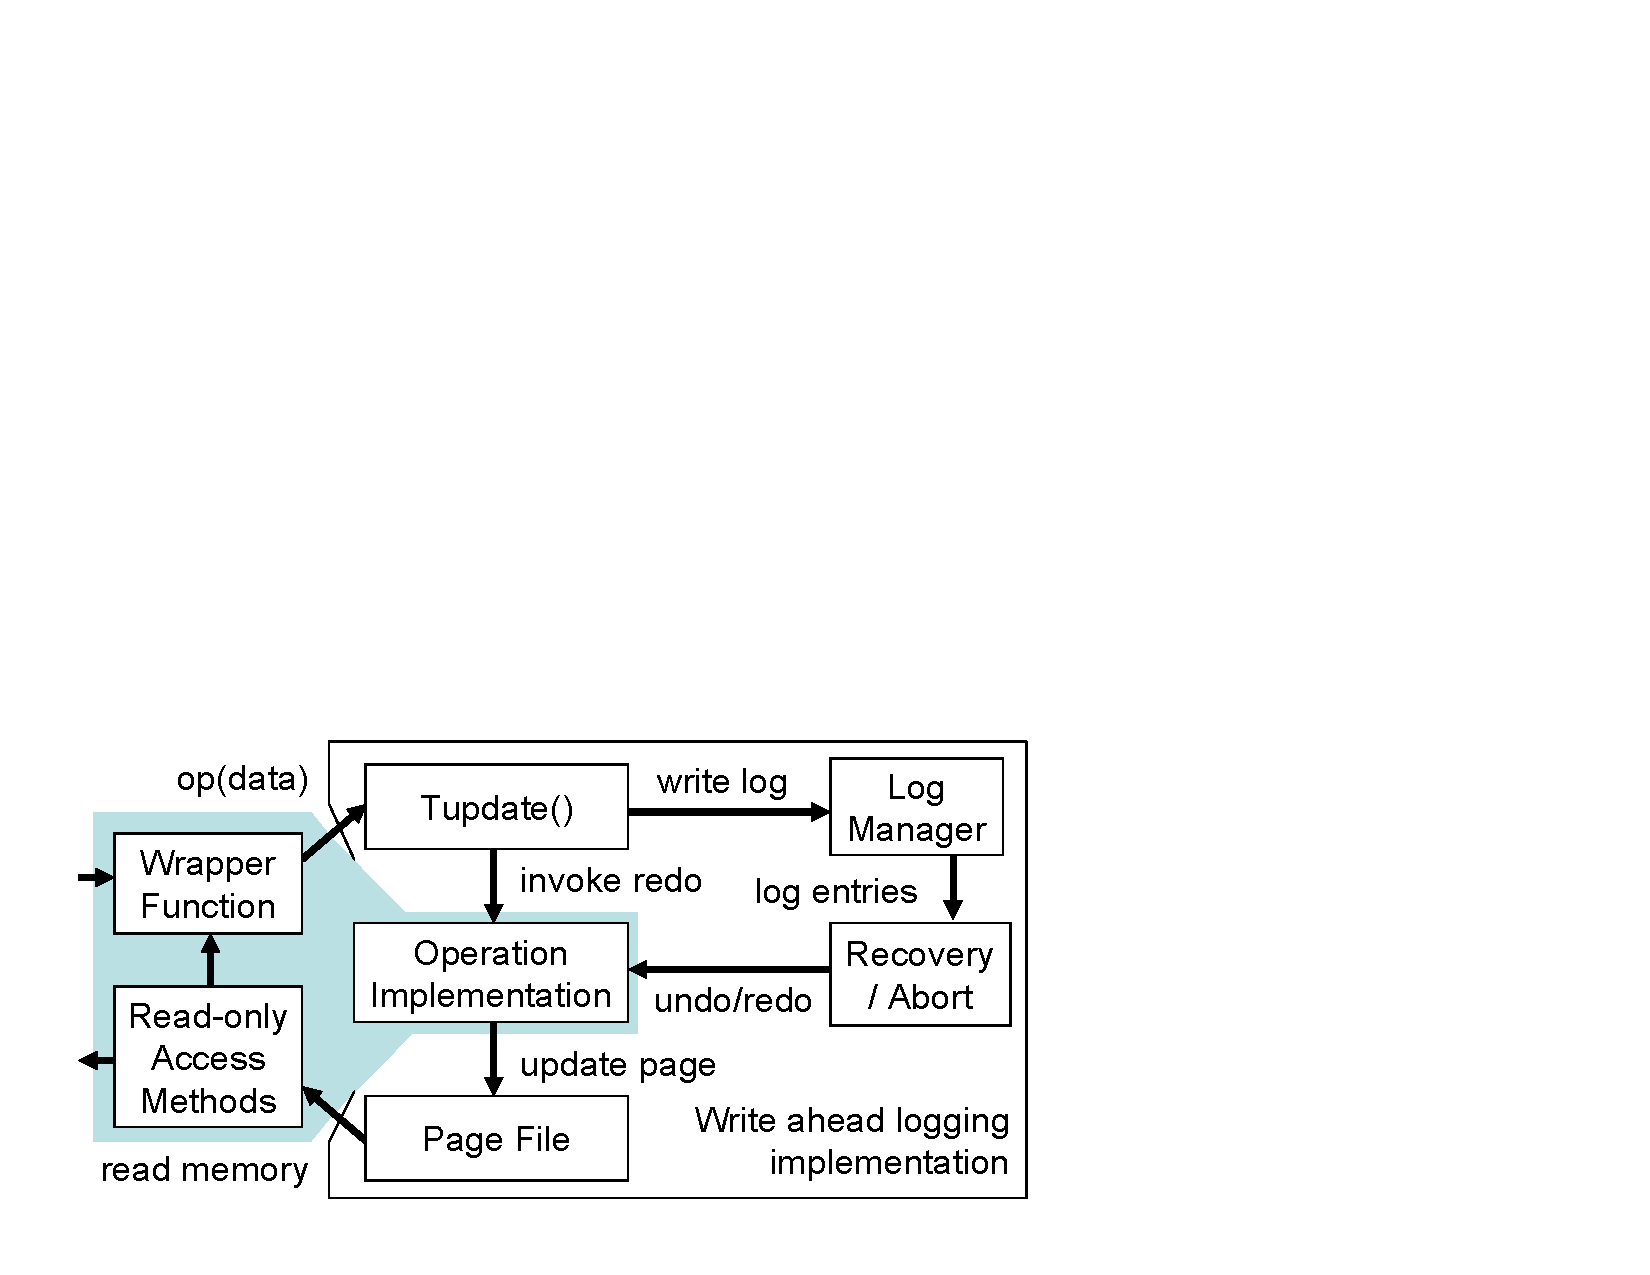
\includegraphics[%
   width=1\columnwidth]{figs/structure.pdf}
\caption{\sf\label{fig:structure} The portions of \yad that new operations interact with directly.}
\end{figure}
\yad allows application developers to easily add new operations to the
system.  Many of the customizations described below can be implemented
using custom log operations.  In this section, we desribe how to add a
``typical'' Steal/no-Force operation that supports concurrent
transactions, full physiological logging, and per-page LSN's.  Such
opeartions are typical of high-performance commercial database
engines.

As we mentioned above, \yad operations must implement a number of
functions.  Figure~\ref{yadArch} describes the environment that
schedules and invokes these functions.  The first step in implementing
a new set of log interfaces is to decide upon interface that these log
interfaces will export to callers outside of \yad.  

These interfaces are implemented by the Wrapper Functions and Read
only access methods in Figure~\ref{yadArch}.  Wrapper functions that
modify the state of the database package any information that will be
needed for undo or redo into a data format of its choosing.  This data
structure, and an opcode associated with the type of the new
operation, are passed into Tupdate(), which copies its arguments to
the log, and then passes its arguments into the operation's REDO
function.
 
REDO modifies the page file, or takes some other action directly.  It
is essentially an iterpreter for the log entries it is associated
with.  UNDO works analagously, but is invoked when an operation must
be undone (usually due to an aborted transaction, or during recovery).
This general pattern is quite general, and applies in many cases.  In
order to implement a ``typical'' operation, the operations
implementation must obey a few more invariants:

\begin{itemize}
\item Pages should only be updated inside REDO and UNDO functions.
\item Page updates atomically update page LSN's by pinning the page.
\item If the data seen by a wrapper function must match data seen
  during REDO, then the wrapper should use a latch to protect against
  concurrent attempts to update the sensitive data (and against
  concurrent attempts to allocate log entries that update the data).
\item Nested top actions (and logical undo), or ``big locks'' (which
  reduce concurrency) should be used to implement multi-page updates.
\end{itemize}

\subsection{Linear hash table}
\begin{figure}[t]
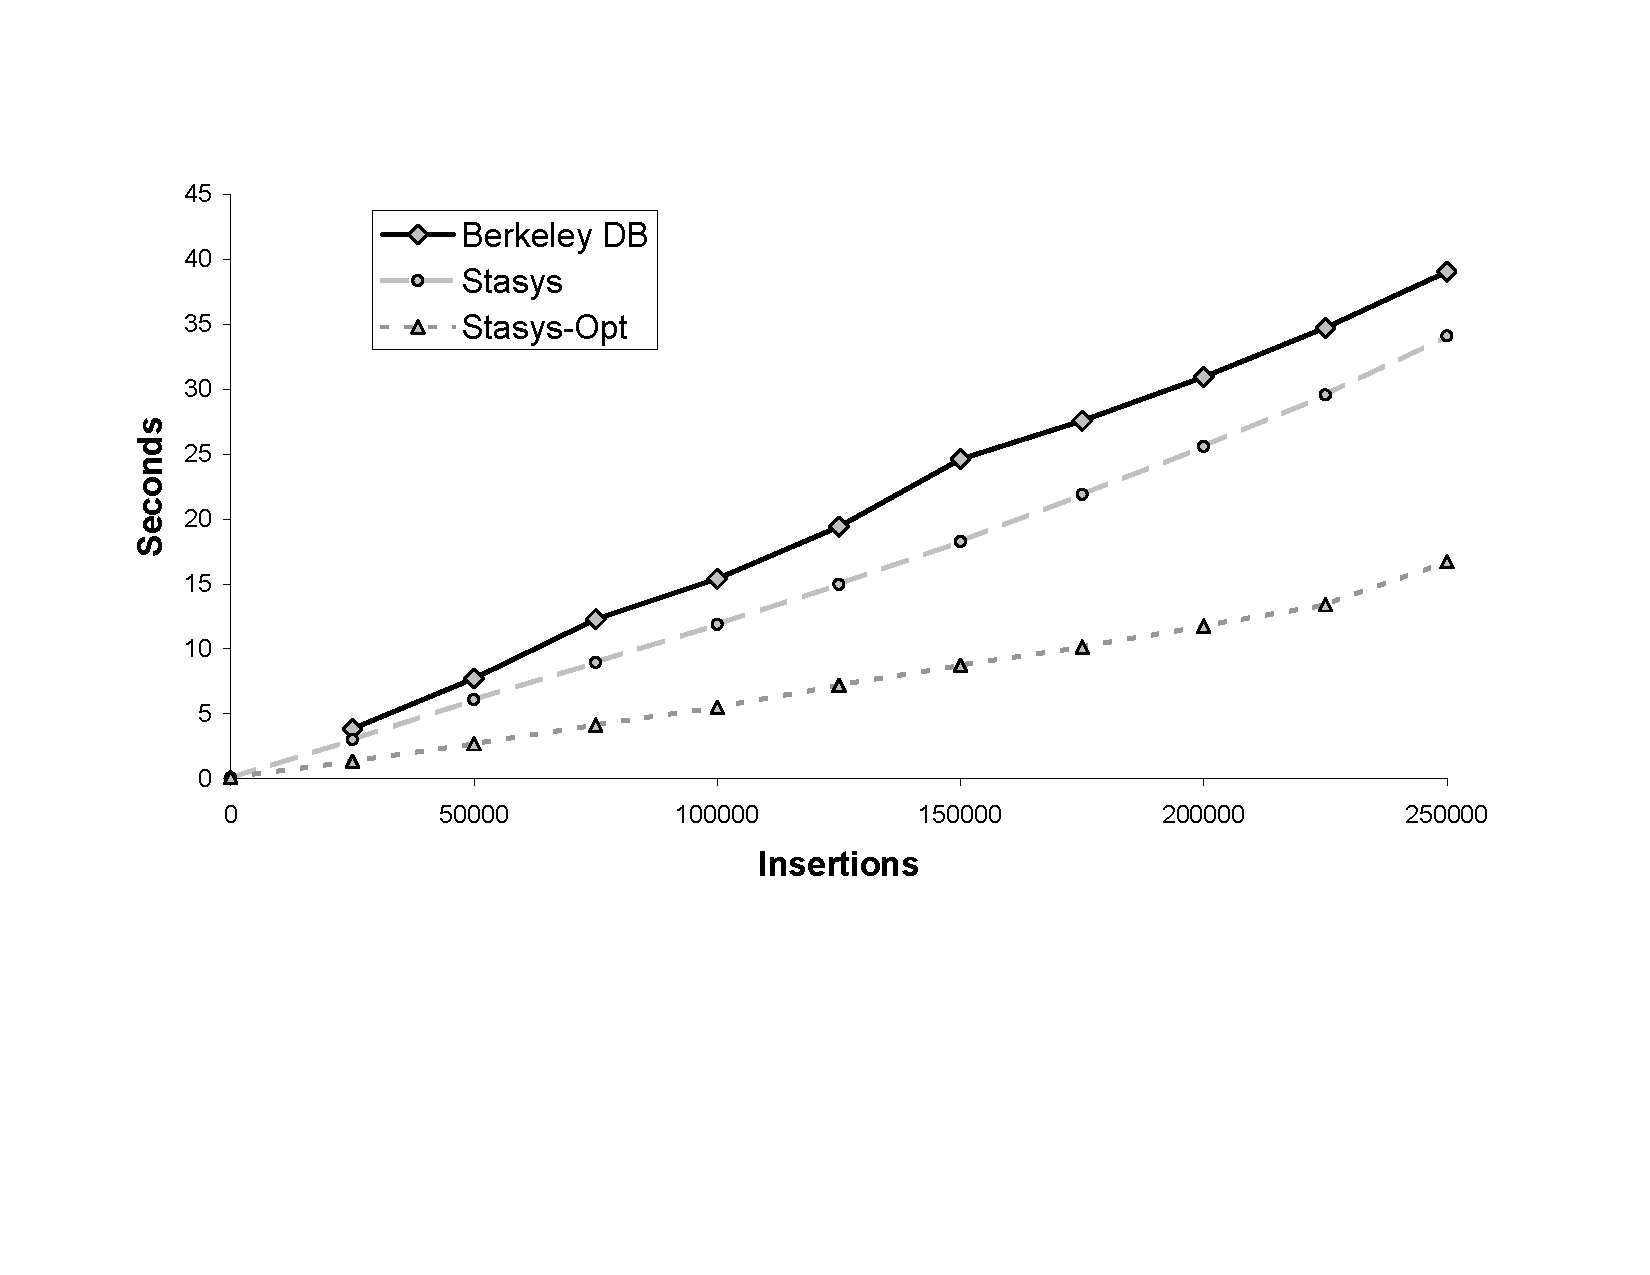
\includegraphics[%
   width=1\columnwidth]{figs/bulk-load.pdf}
%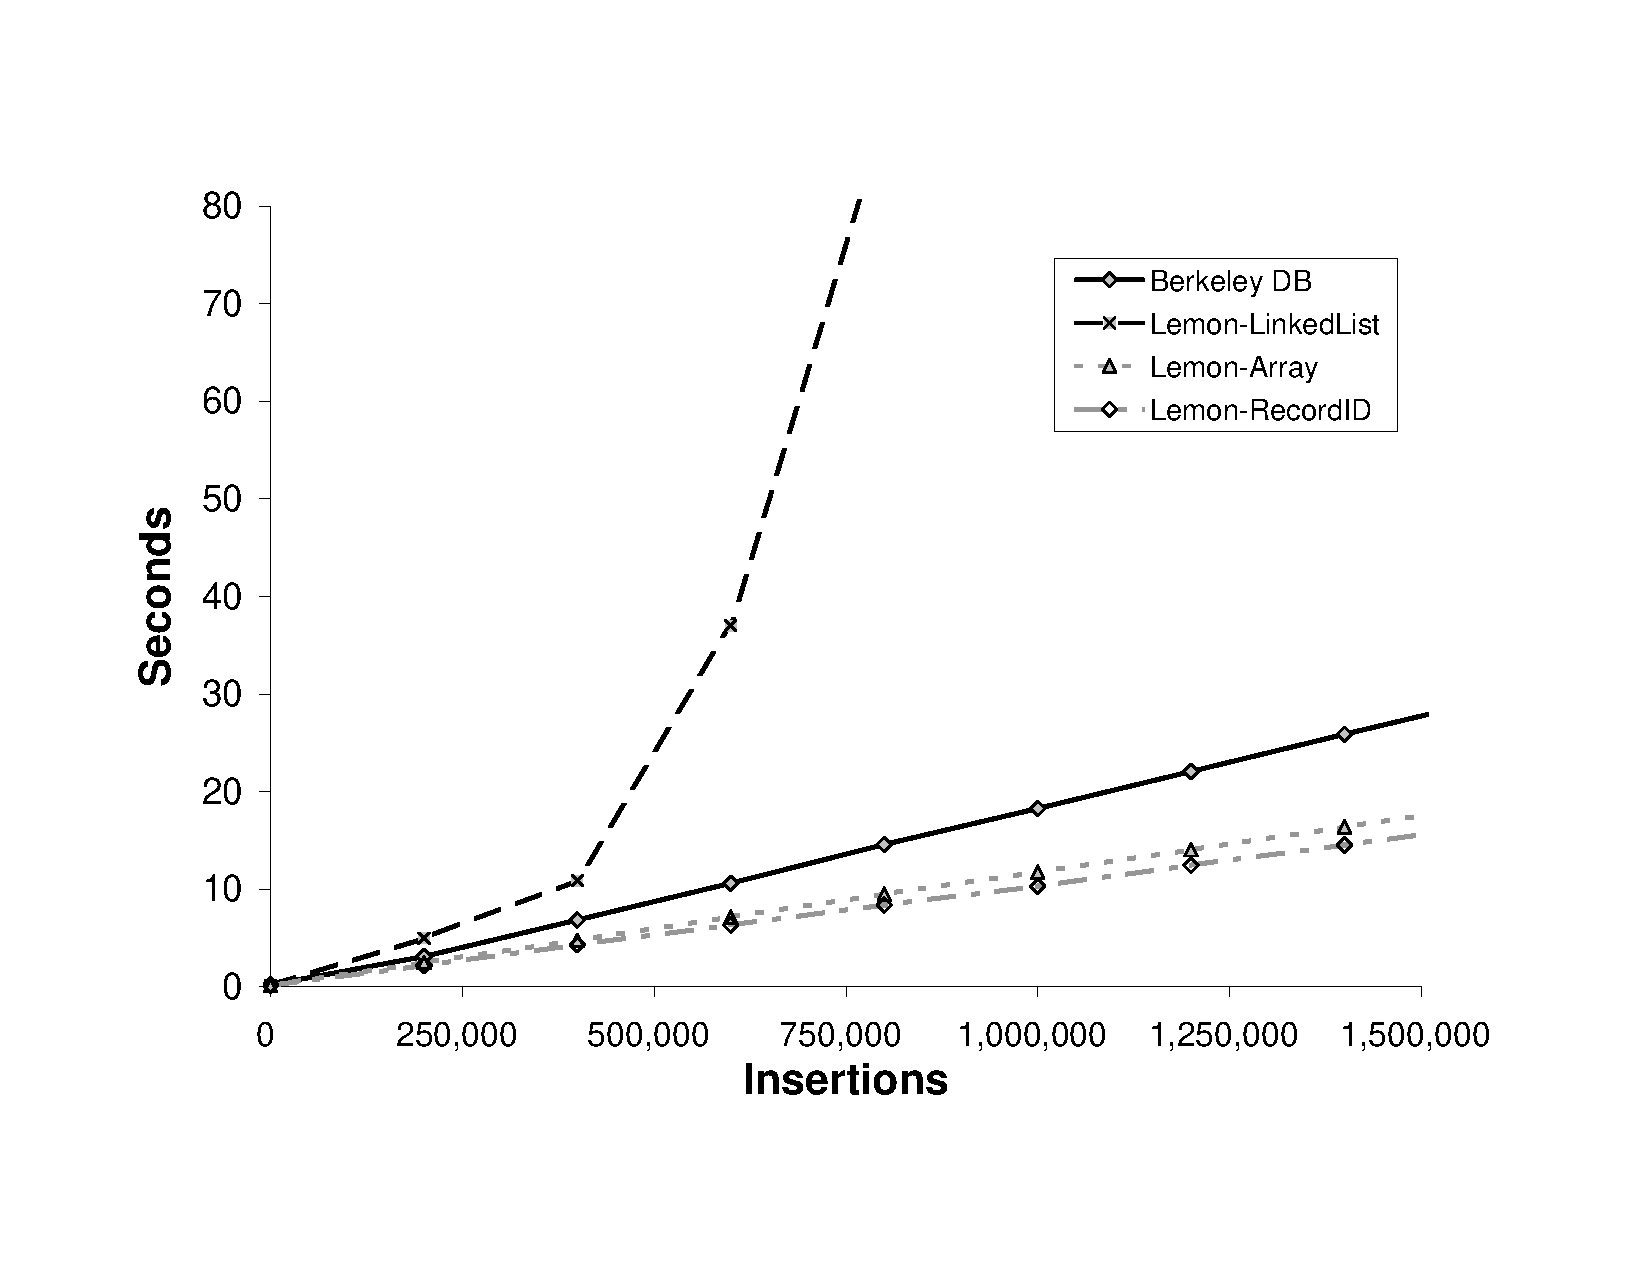
\includegraphics[%
%   width=1\columnwidth]{bulk-load-raw.pdf}
%\vspace{-30pt}
\caption{\sf\label{fig:BULK_LOAD} Performance of \yad and Berkeley DB hashtable implementations.  The
test is run as a single transaction, minimizing overheads due to synchronous log writes.}
\end{figure}
\begin{figure}[t]
%\hspace*{18pt}
%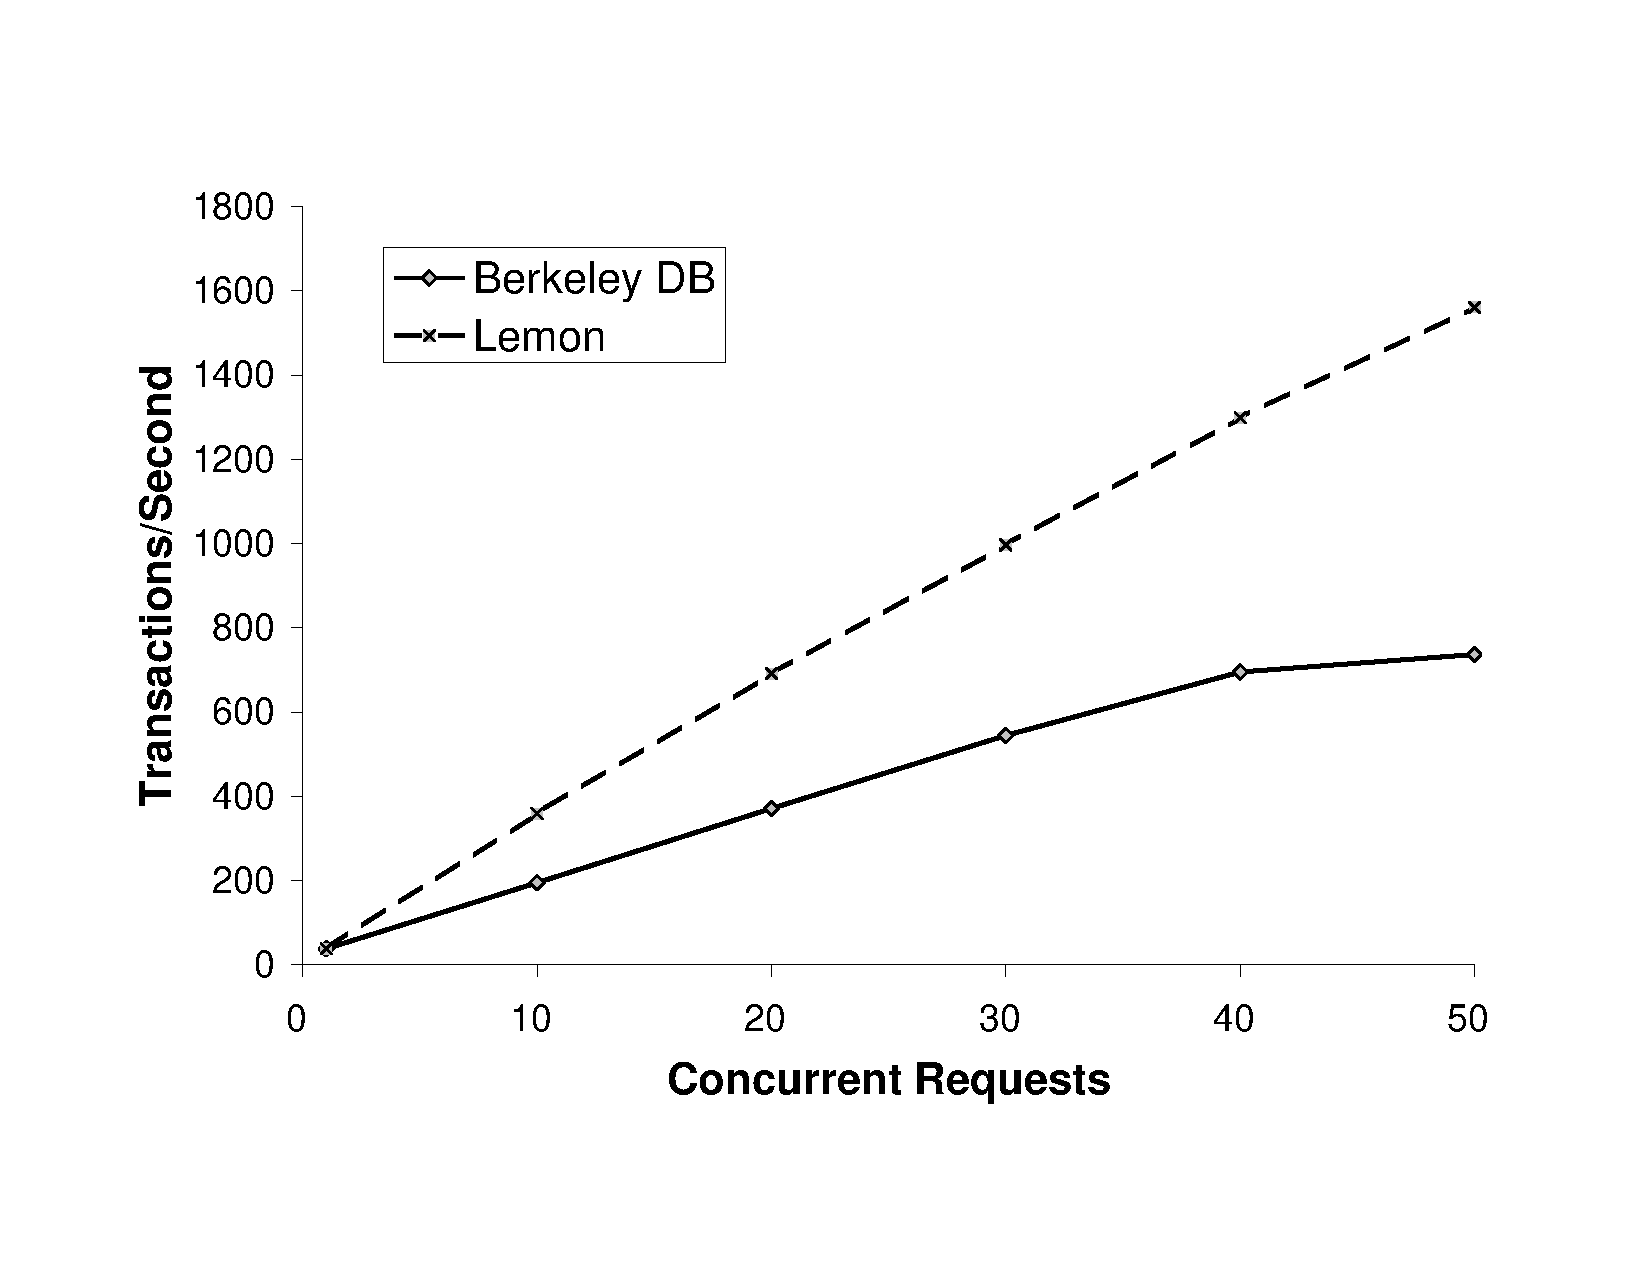
\includegraphics[%
%   width=1\columnwidth]{tps-new.pdf}
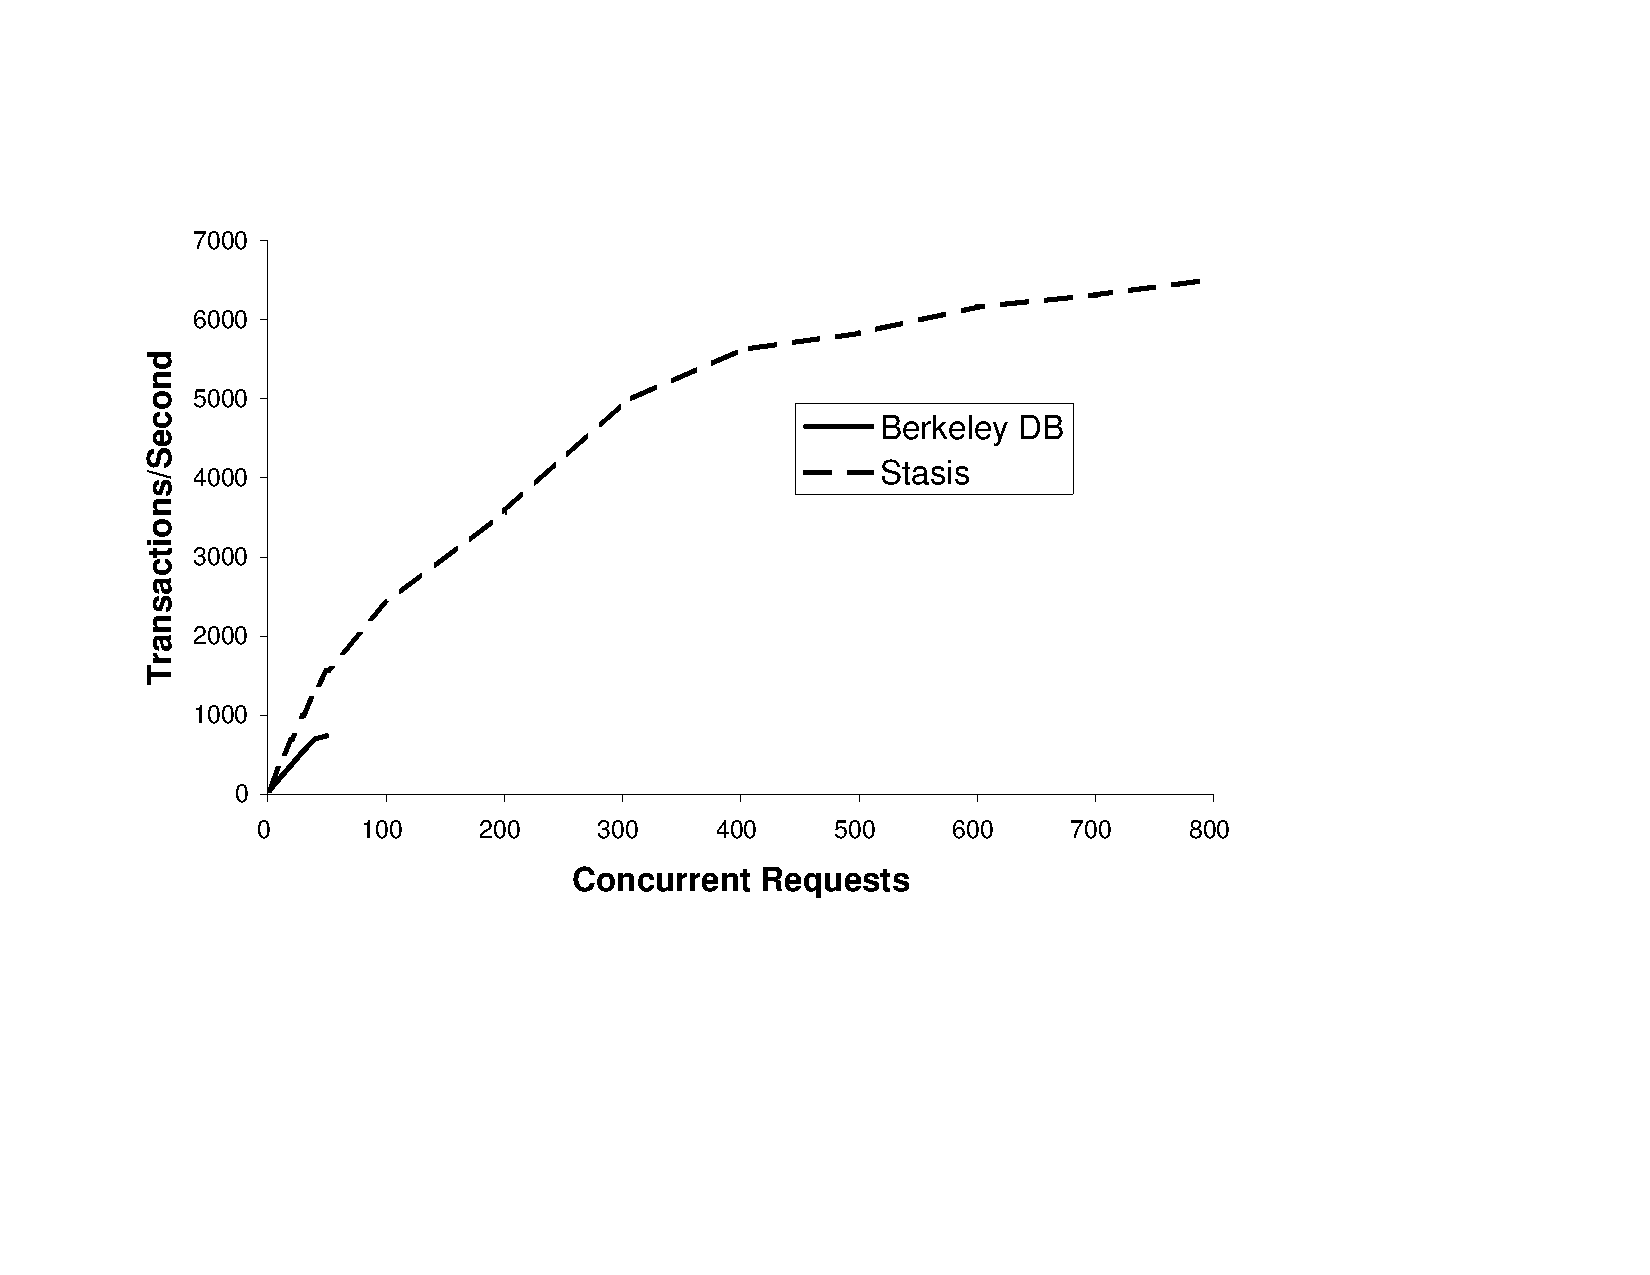
\includegraphics[%
   width=3.25in]{figs/tps-extended.pdf}
%\vspace{-36pt}
\caption{\sf\label{fig:TPS} High concurrency performance of Berkeley DB and \yad.  We were unable to get Berkeley DB to work correctly with more than 50 threads. (See text)
}
\end{figure}

Although the beginning of this paper describes the limitations of
physical database models and relational storage systems in great
detail, these systems are the basis of most common transactional
storage routines.  Therefore, we implement key-based storage, and a
primititve form of linksets in this section.  We argue that obtaining
obtaining reasonable performance in such a system under \yad is
straightforward, and compare a simple hash table to a hand-tuned (not
straightforward) hash table, and Berkeley DB's implementation.

The simple hash table uses nested top actions to atomically update its
internal structure.  It is based on a linear hash function, allowing
it to incrementally grow its buffer list.  It is based on a number of
modular subcomponents, notably a growable array of fixed length
entries, and the user's choice of two different linked list
implementations.  The hand-tuned hashtable also uses a {\em linear} hash
function,~\cite{lht} but is monolithic, and uses carefully ordered writes to
reduce log bandwidth, and other runtime overhead.  Berkeley DB's
hashtable is a popular, commonly deployed implementation, and serves
as a baseline for our experiements.

Both of our hashtables outperform Berkeley DB on a workload that
bulkloads the tables by repeatedly inserting key, value pairs into
them.  We do not claim that our partial implementation of \yad
generally outperforms Berkeley DB, or that it is a robust alternative
to Berkeley DB.  Instead, this test shows that \yad is comparable to
existing systems, and that its modular design does not introduce gross
inefficiencies at runtime.

The comparison between our two hash implementations is more
enlightening.  The performance of the simple hash table shows that
quick, straightfoward datastructure implementations composed from
simpler structures behave reasonably well in \yad.  The hand-tuned
implementation shows that \yad allows application developers to
optimize the primitives they build their applications upon.  In the
best case, past systems allowed application developers to providing
hints to improve performance.  In the worst case, a developer would be
forced to redesign the application to avoid sub-optimal properties of
the transactional data structure implementation.

Figure~\ref{lhtThread} describes performance of the two systems under
highly concurrent workloads.  For this test, we used the simple
(unoptimized) hash table, since we are interested in the performance a
clean, modular data structure that a typical system implementor would
be likely to produce, not the performance of our own highly tuned,
monolithic, implementations.

Both Berekely DB and \yad can service concurrent calls to commit with
a single synchronous I/O.\endnote{The multi-threaded benchmarks
  presented here were performed using an ext3 filesystem, as high
  concurrency caused both Berkeley DB and \yad to behave unpredictably
  when reiserfs was used.  However, \yad's multi-threaded throughput
  was significantly better that Berkeley DB's under both systems.}
\yad scaled quite well, delivering over 6000 transactions per
second,\endnote{This test was run without lock managers, so the
  transactions obeyed the A, C, and D properties.  Since each
  transaction performed exactly one hashtable write and no reads, they
  obeyed I (isolation) in a trivial sense.}  and provided roughly
double Berkeley DB's throughput (up to 50 threads).  We do not report
the data here, but we implemented a simple load generator that makes
use of a fixed pool of threads with a fixed think time.  We found that
the latency of Berkeley DB and \yad were similar, addressing concerns
that \yad simply trades latency for throughput during the concurrency
benchmark.

\subsection{Object serialization}

\begin{figure*}[t!]
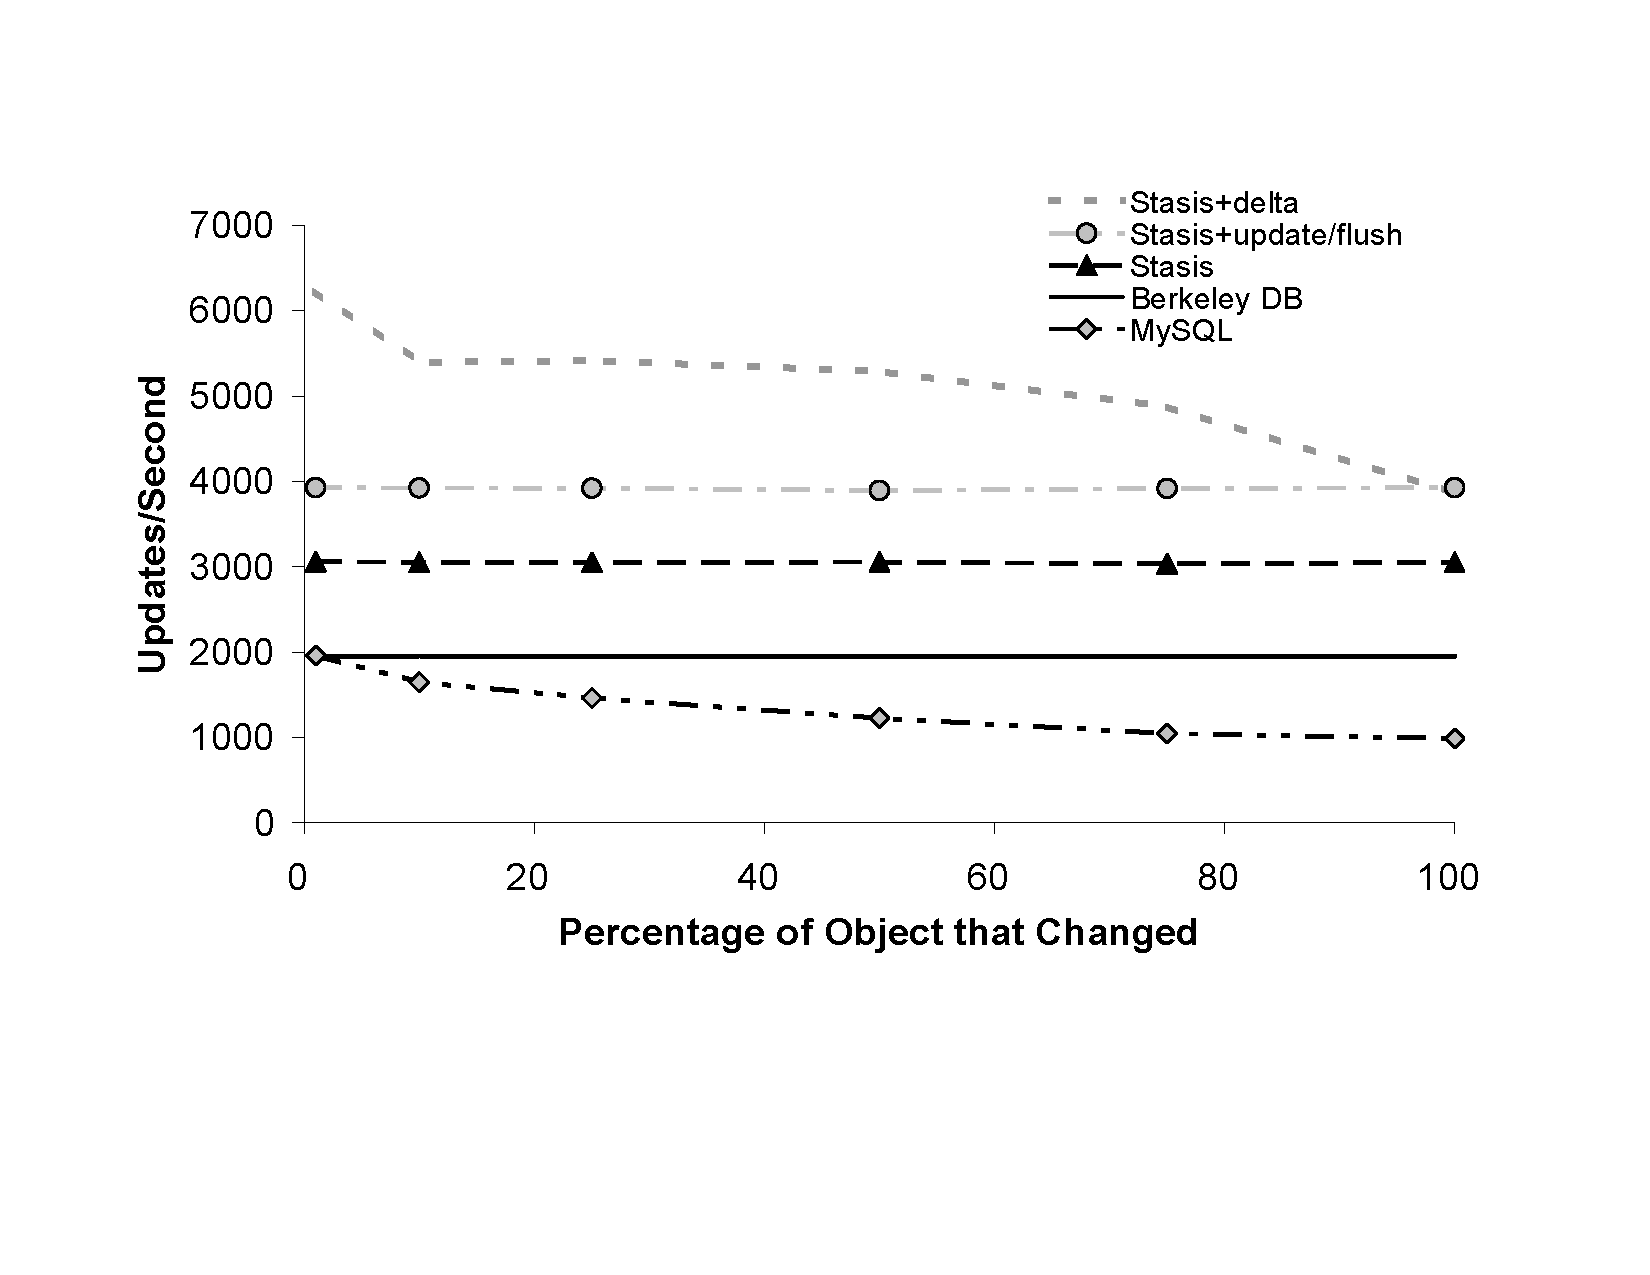
\includegraphics[width=3.3in]{figs/object-diff.pdf}
\hspace{.3in}
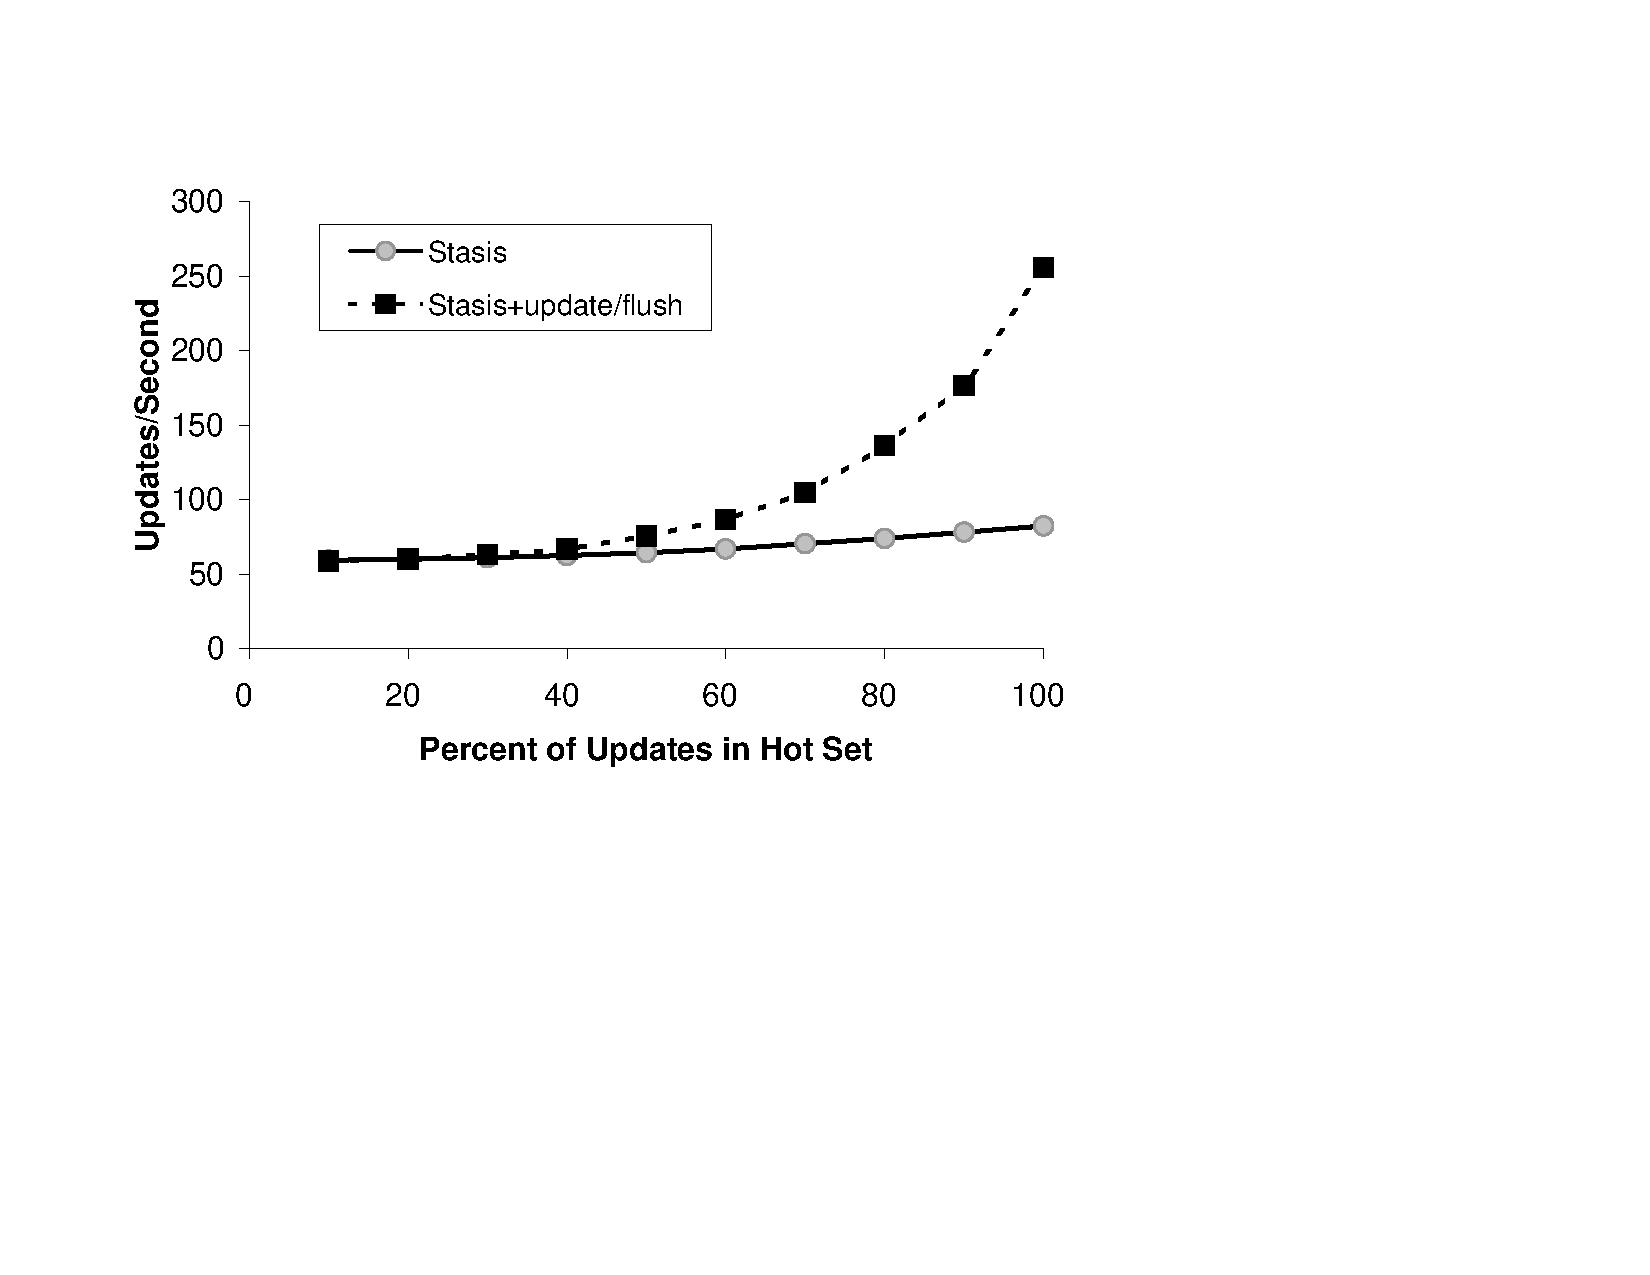
\includegraphics[width=3.3in]{figs/mem-pressure.pdf}
\vspace{-.15in}
\caption{\sf \label{fig:OASYS}
The effect of \yad object serialization optimizations under low and high memory pressure.}
\end{figure*}

Numerous schemes are used for object serialization.  Support for two
different styles of object serialization have been eimplemented in
\yad.  The first, pobj, provided transactional updates to objects in
Titanium, a Java variant.  It transparently loaded and persisted
entire graphs of objects.

The second variant was built on top of a generic C++ object
serialization library, \oasys.  \oasys makes use of pluggable storage
modules to actually implement persistant storage, and includes plugins
for Berkeley DB and MySQL.  This section will describe how the \yad's
\oasys plugin reduces the runtime serialization/deserialization cpu
overhead of write intensive workloads, while using half as much system
memory as the other two systems.

We present three variants of \yad here.  The first treats \yad like
Berkeley DB.  The second customizes the behavior of the buffer
manager.  Instead of maintaining an up-to-date version of each object
in the buffer manager or page file, it allows the buffer manager's
view of live application objects to become stale.  This is safe since
the system is always able to reconstruct the appropriate page entry
form the live copy of the object.

The reason it would be difficult to do this with Berkeley DB is that
we still need to generate log entries as the object is being updated.
Otherwise, commit would not be durable, and the application would be
unable to abort() transactions.  Even if we decided to disallow
application aborts, we would still need to write log entries
committing.  This would cause Berekley DB to write data back to the
page file, increasing the working set of the program, and increasing
disk activity.

Under \yad, we implemented this optimization by adding two new
operations, update(), which only updates the log, and flush(), which
updates the page file.  We decrease the size of the page file, so
flush() is likely to incur disk overhead.  However, we have roughly
doubled the number of objects that are cached in memory, and expect
flush() to be called relatively infrequently.

The third \yad plugin to \oasys incorporated all of the updates of the
second, but arranged to only the changed portions of objects to the
log.

Figure~\ref{objectSerialization} presents the performance of the three
\yad optimizations, and the \oasys plugins implemented on top of other
systems.  As we can see, \yad performs better than the baseline
systems.  More interestingly, in non-memory bound systems, the
optimizations nearly double \yad's performance, and we see that in the
memory-bound setup, update/flush indeed improves memory utilization.


\subsection{Manipulation of logical log entries}

\begin{figure}
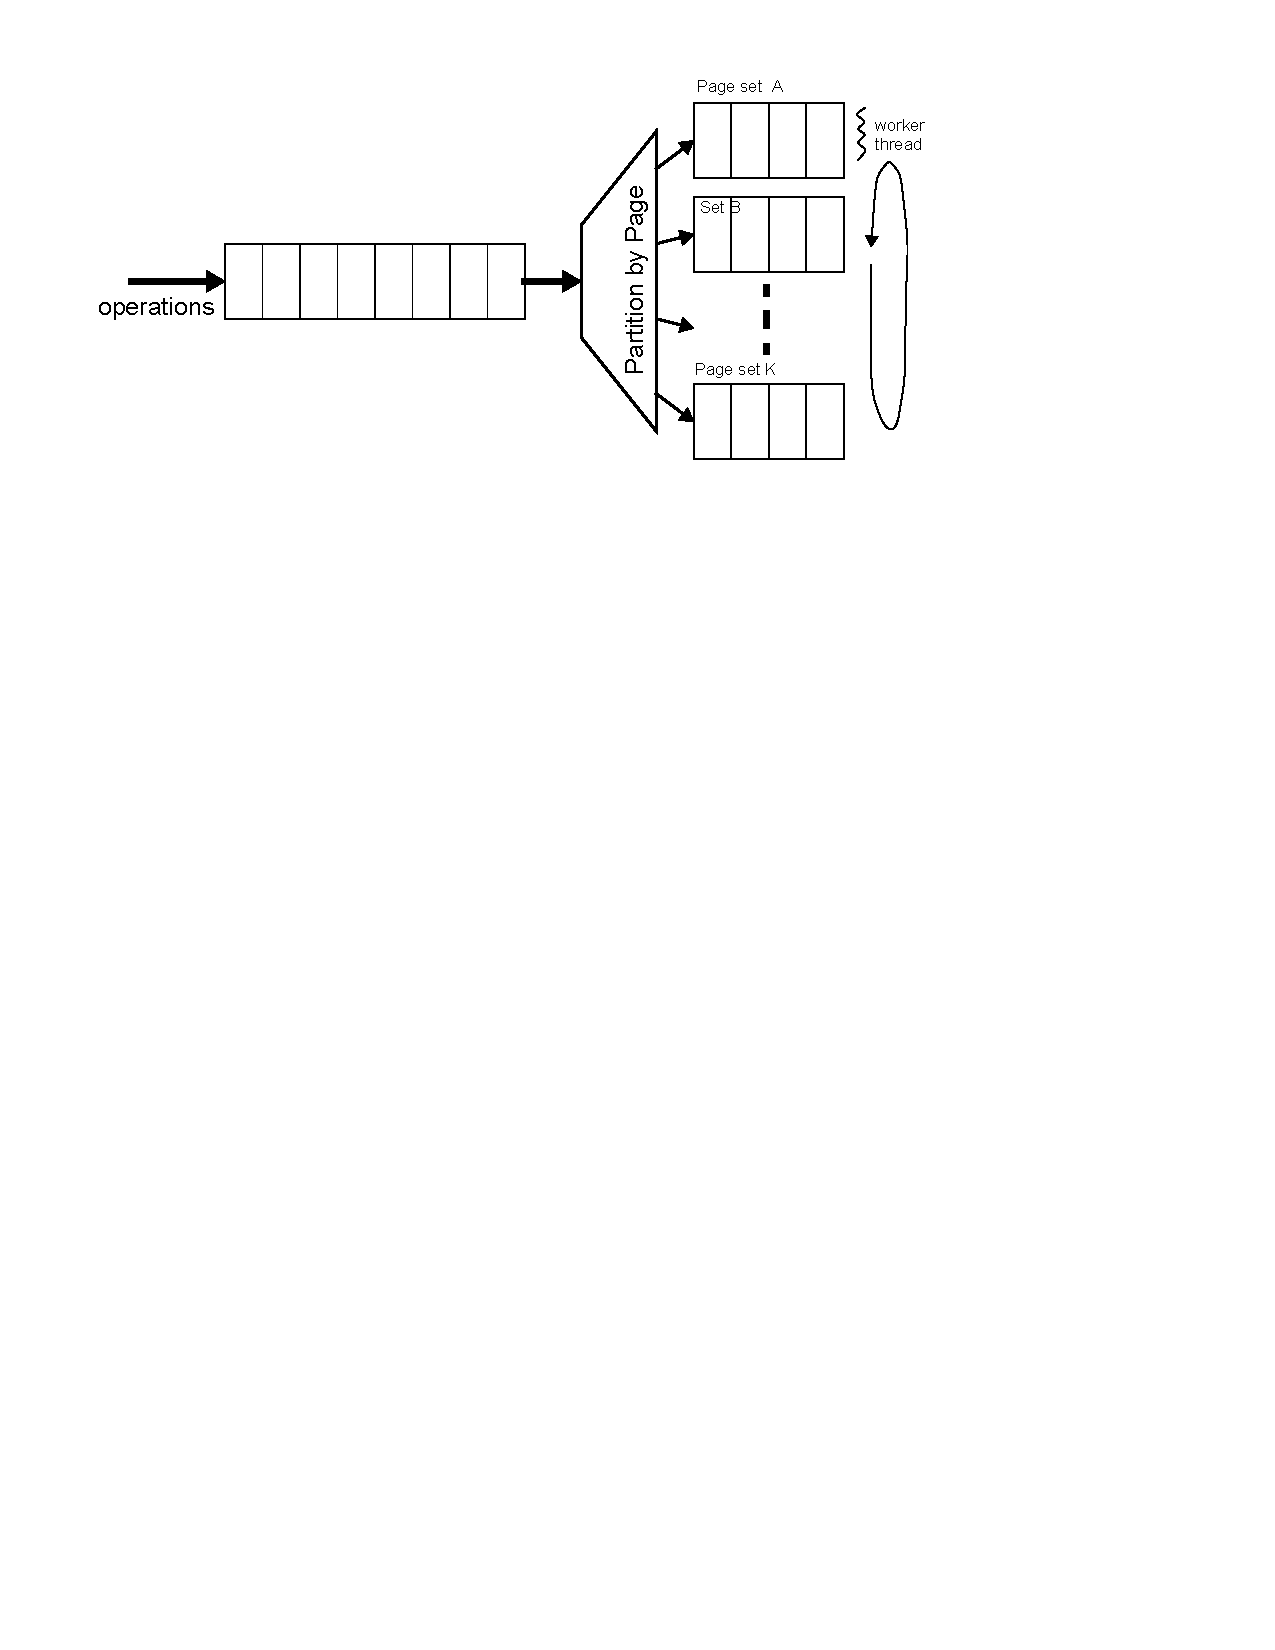
\includegraphics[width=1\columnwidth]{figs/graph-traversal.pdf}
\vspace{-24pt}
\caption{\sf\label{fig:multiplexor} Because pages are independent, we
can reorder requests among different pages. Using a log demultiplexer,
we partition requests into independent queues, which can be 
handled in any order, improving locality and merging opportunities.}
\end{figure}
\begin{figure}[t]
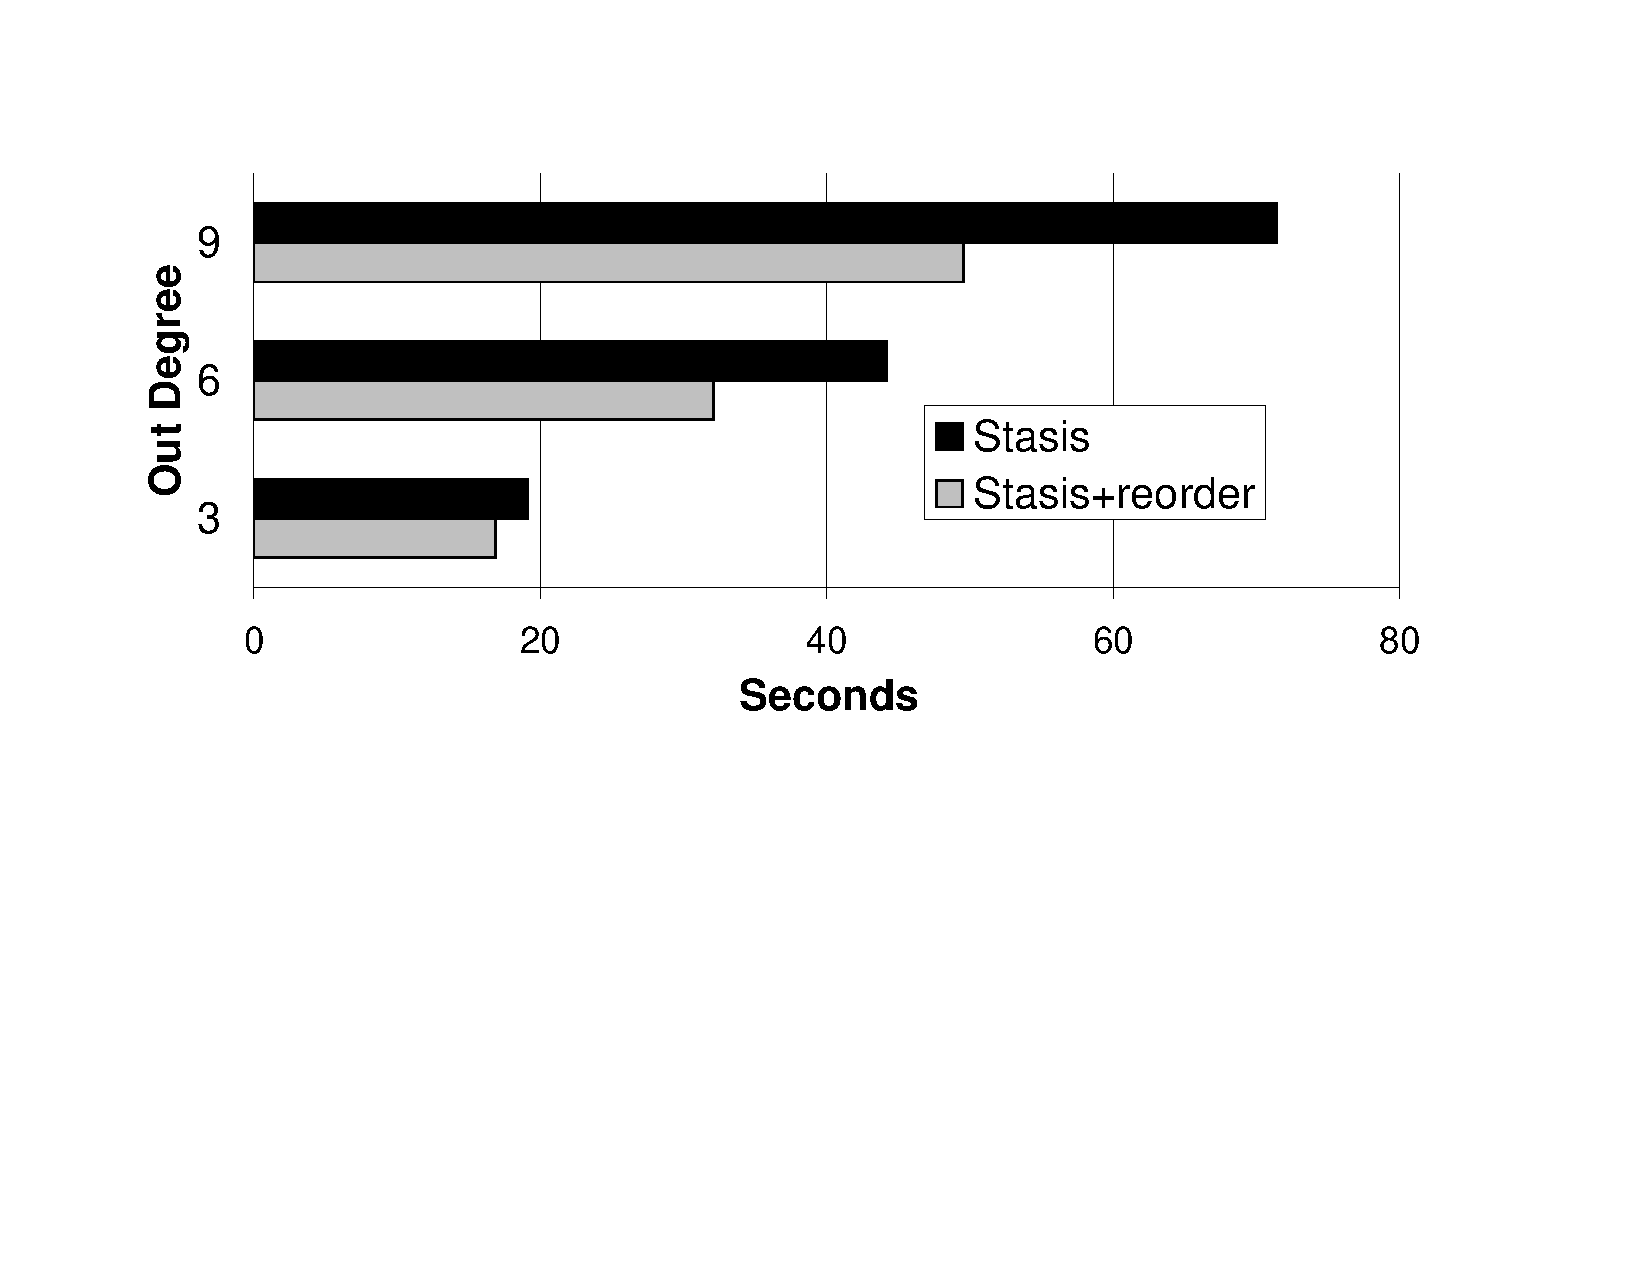
\includegraphics[width=3.3in]{figs/oo7.pdf}
\vspace{-15pt}
\caption{\sf\label{fig:oo7} oo7 benchmark style graph traversal.  The optimization performs well due to the presence of non-local nodes.}
\end{figure}

\begin{figure}[t]
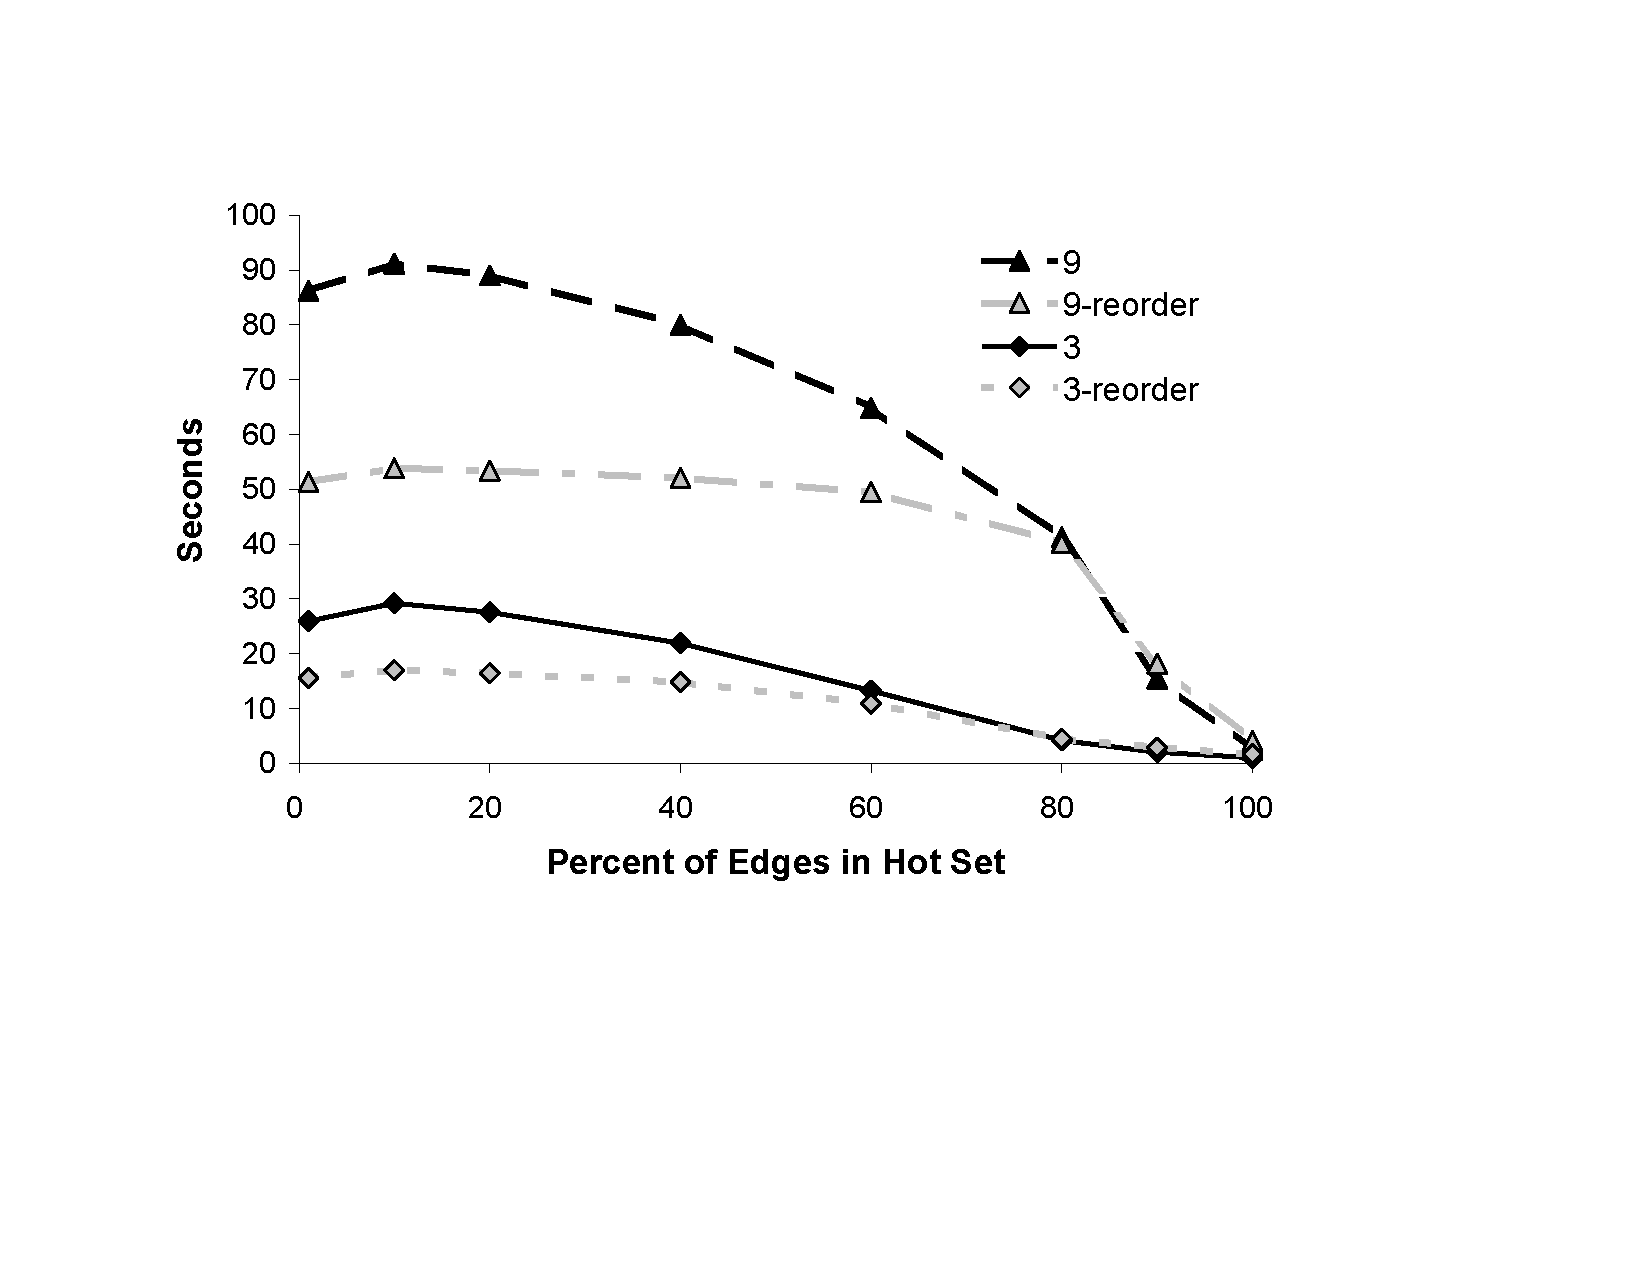
\includegraphics[width=3.3in]{figs/trans-closure-hotset.pdf}
\vspace{-12pt}
\caption{\sf\label{fig:hotGraph} Hot set based graph traversal for random graphs with out-degrees of 3 and 9.  Here
we see that the multiplexer helps when the graph has poor locality.
However, in the cases where depth first search performs well, the
reordering is inexpensive.}
\end{figure}

Database optimizers operate over relational algebra expressions that
will correspond to sequence of logical operations at runtime.  \yad
does not support query languages, relational algebra, or other general
purpose primitves.

However, it does include an extendible logging infrastructure, and any
operations that make user of physiological logging implicitly
implement UNDO (and often REDO) functions that interpret logical
operations.

Logical operations often have some nice properties that this section
will exploit.  Because they can be invoked at arbitrary times in the
future, they tend to be independent of the database's physical state.
They tend to be inverses of operations that programmer's understand.
If each method in the API exposed to the programmer is the inverse of
some other method in the API, then each logical operation corresponds
to a method the programmer can manually invoke.

Because of this, application developers can easily determine whether
logical operations may safely be reordered, transformed, or even
dropped from the stream of requests that \yad is processing.  Even
better, if requests can be partitioned in a natural way, load
balancing can be implemented by spliting requests across many nodes.
Similarly, a node can easily service streams of requests from multiple
nodes by combining them into a single log, and processing the log
using operaiton implementations.  Furthermore, application-specific
procedures that are analagous to standard relational algebra methods
(join, project and select) could be used to efficiently transform the data
before it reaches the page file, while it is layed out sequentially
in memory.

Note that read-only operations do not necessarily generate log
entries.  Therefore, applications may need to implement custom
operations to make use of the ideas in this section.

Although \yad has rudimentary support for a two-phase commit based
cluster hash table, we have not yet implemented a logical log based
networking primitives.  Therefore, we implemented some of these ideas
in a single node configuration in order to increase request locality
during the traversal of a random graph.  The graph traversal system
takes a sequence of (read) requests, and partitions them using some
function.  It then proceses each partition in isolation from the
others.  We considered two partitioning functions.  The first, which
is really only of interested in the distributed case, partitions the
requests according to the hash of the node id they refer to.  This
would allow us to balance the graph traversal across many nodes.  (We
expect the early phases of such a traversal to be bandwidth, not
latency limited, as each node would stream large sequences of
asynchronous requests to the other nodes.) 

The second partitioning function, which was used to produce
Figure~\ref{hotset} partitions requests by their position in the page
file.  When the graph has good locality, a normal depth first search
traversal and the prioritized traversal perform well.  As locality
decreases, the partitioned traversal algorithm's performance degrades
less than the naive traversal.

**TODO This really needs more experimental setup... look at older draft!**

\subsection{LSN-Free pages}

In Section~\ref{todo}, we describe how operations can avoid recording
LSN's on the pages they modify.  Essentially, opeartions that make use
of purely physical logging need not heed page boundaries, as
physiological operations must.  Recall that purely physical logging
interacts poorly with concurrent transactions that modify the same
data structures or pages, so LSN-Free pages are not applicable in all
situations.

Consider the retreival of a large (page spanning) object stored on
pages that contain LSN's.  The object's data will not be contiguous.
Therefore, in order to retrive the object, the transaction system must
load the pages contained on disk into memory, allocate buffer space to
allow the object to be read, and perform a byte-by-byte copy of the
portions of the pages that contain the large object's data.  Compare
this approach to a modern filesystem, which allows applications to
perform a DMA copy of the data into memory, avoiding the expensive
byte-by-byte copy of the data, and allowing the CPU to be used for
more productive purposes.  Furthermore, modern operating systems allow
network services to use DMA and ethernet adaptor hardware to read data
from disk, and send it over a network socket without passing it
through the CPU.  Again, this frees the CPU, allowing it to perform
other tasks.

We beleive that LSN free pages will allow reads to make use of such
optimizations in a straightforward fashion.  Zero copy writes could be
performed by performing a DMA write to a portion of the log file.
However, doing this complicates log truncation, and does not address
the problem of updating the page file.  We suspect that contributions
from the log based filesystem literature can address these problems in
a straightforward fashion.

Finally, RVM, recoverable virtual memory, made use of LSN-free pages
so that it could use mmap() to map portions of the page file into
application memory.  However, without support for logical log entries
and nested top actions, it would be difficult to implement a
concurrent, durable data structure using RVM.  We plan to add RVM
style transactional memory to \yad in a way that is compatible with
fully concurrent collections such as hash tables and tree structures.

\section{Conclusion}

\section{Acknowledgements}

\section{Availability}

Additional information, and \yad's source code is available at:

\begin{center}
{\tt http://\yad.sourceforge.net/}
\end{center}

{\footnotesize \bibliographystyle{acm}
\nocite{*}
\bibliography{LLADD}}

\theendnotes

\end{document}







